\begin{section}{Method}
  \label{sec:method}

In our study we make use of the N-body simulation code 
\cpm{} and follow the implementation in \cite{bib:Inman}. 
For generating initial conditions, we use density transfer 
functions, $T_\delta$ obtained from \camb{}. The initial 
velocities of the neutrinos are comprised of a linear 
and thermal part. To compute the former, we assume that 
the initial conditions are adiabatic and linear 
so that we may use the linear neutrino velocity transfer 
function defined as
\begin{equation}
  T_v=-i\frac{H}{k}\frac{dT_{\delta}}{dz}
\end{equation}
From this, a velocity potential $\phi_{v}(k)$ satisfying 
$i\overrightarrow{k}\phi_{v}(k)=(T_v/T_\delta)\delta\hat{k}$ 
is obtained from which the linear velocity may be computed 
using a real-space gradient. The thermal component of the 
velocity is calculated using the relativistic Fermi-Dirac distribution. 

\par To limit slowdown of the simulation, cold dark matter is 
introduced at $z=100$ whereas neutrinos are introduced 
at $z=10$. The two species are then allowed to evolve together 
identically up to $z=0$, save for their masses which are weighted by their
energy fraction and number ratio. Additionally, at $z=10$ we 
divide the neutrinos into four bins - $Q_i$, $i=1,2,3,4$ - based 
on their velocity such that each bin contains an equal 
number of particles as per the Fermi-Dirac distribution (e.g. 
$Q_1$ contains neutrinos whose velocities are in the first quartile). 
The lower bounds used for these velocity bins 
are: $0\,\kms{}, 5214\,\kms{}, 7853\, \kms{}, 11280\,\kms{}$. 
In order to determine at later times in which velocity bin 
each neutrino began, a unique 8-byte particle identifier tag is 
assigned to each neutrino. 

% Velocity Fields
\par In order to compute the dipole correlation function at $z=0$, we
 must first calculate the density and velocity fields. The 
former is determined for both neutrinos and dark matter 
using a cloud-in-cell method. Calculation of the 
velocity field for neutrinos is done by dividing their 
momentum field by their density field using a coarsened grid.

\par In practice, however, the neutrino velocity field is 
impossible to observe. As such, we also compute the velocity 
field using the density field via linear theory. Following 
the above discussion, we have
\begin{equation}
   \vec{v} = \frac{T_{v}}{T_{\delta}}\frac{\vec{k}}{k}\delta,
\end{equation}
where in our calculations, $\delta$ is the CDM density field. 
As discussed in \cite{bib:Inman}, the linearly reconstructed velocity fields 
give an accurate representation of the actual large-scale velocity 
field in the simulation. In order to apply this reconstruction 
to each neutrino velocity bin, we produce window functions for
each bin as shown in Fig. \ref{fig:fdwindow} using a Fermi-Dirac
distribution. We pass these window functions to \class{} to
produce transfer functions for each bin \cite{bib:Blas}.
%the windows are constructed such that $n_{eff}$ remains constant 
%and is consistent with a neutrino cosmology.

\begin{figure}[tbp]
  \begin{center}
    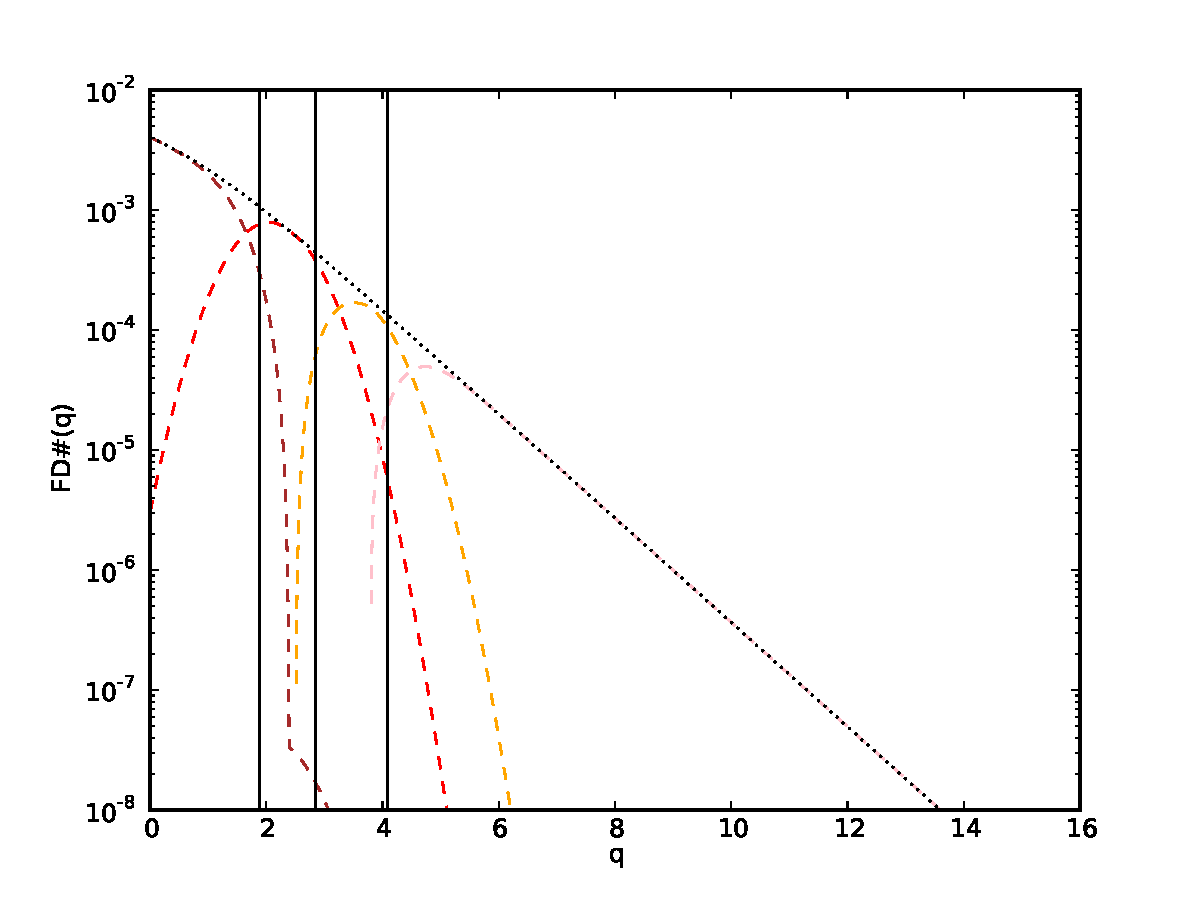
\includegraphics[width=0.5\textwidth]{./figures/fdwindow.pdf}
    \caption{Window functions passed to CLASS to produce transfer functions.
	     Solid black lines indicate the bounds of each velocity bin. The dotted
	     curve indicates the total Fermi-Dirac distribution and the dashed lines
	     are the window functions used for each velocity bin. Here, $m=0.2\ev{}$ and $T$ 
	     are the neutrino mass and temperature, respectively..}
    \label{fig:fdwindow}
  \end{center}
\end{figure}
   
% Dipole Correlation Calculation; leave empty for now

\end{section}
